%% LyX 2.0.4 created this file.  For more info, see http://www.lyx.org/.
%% Do not edit unless you really know what you are doing.
\documentclass[oneside,english,dutch]{amsart}
\usepackage[T1]{fontenc}
\usepackage[latin9]{inputenc}
\usepackage[a4paper]{geometry}
\geometry{verbose,tmargin=3cm,bmargin=3cm,lmargin=2cm,rmargin=2cm}
\setlength{\parskip}{\smallskipamount}
\setlength{\parindent}{0pt}
\usepackage{amsthm}
\usepackage{graphicx}
\graphicspath{{Figures/}}

\makeatletter
%%%%%%%%%%%%%%%%%%%%%%%%%%%%%% Textclass specific LaTeX commands.
\numberwithin{equation}{section}
\numberwithin{figure}{section}

\makeatother

\usepackage{babel}
\begin{document}

\title{Data verwerking met periodieke afhankelijkheden}


\author{N.G. Schultheiss}

\maketitle

\section{Inleiding}

Het is mogelijk om gegevens van http://data.hisparc.nl te halen. In
deze module wordt uitgelegd hoe deze gegevens eenvoudig in een spreadsheet
programma kunnen worden ingevoerd.


\section{Het ophalen van data}

\begin{figure}[h]
\includegraphics[width=17cm]{\string"Screenshot-HiSPARC Public Database\string".png}

\caption{Het scherm van http://data.hisparc.nl}
\end{figure}


In figuur 1 is het bovenste deel van het scherm van http://data.hisparc.nl
te zien. Hierin staat een histogram met het aantal co�ncidenties in
een uur tegen de tijd uitgezet. Deze informatie is ook als .csv (comma
separated values) bestand op te halen door op ``source'' rechtsboven
het histogram te klikken. In het bovenstaande scherm krijgen we dan
het bestand in figuur 2.

\begin{figure}
\selectlanguage{english}%
\noindent \begin{raggedright}
\texttt{\scriptsize ;;\textquotedbl{}HiSPARC eventtime histogram source\textquotedbl{}}
\par\end{raggedright}{\scriptsize \par}

\noindent \begin{raggedright}
\texttt{\scriptsize ;;\textquotedbl{}Please note: the 'bin' is the
left bin edge. The width of the bin is 1\textquotedbl{}}
\par\end{raggedright}{\scriptsize \par}

\noindent \begin{raggedright}
\texttt{\scriptsize ;;\textquotedbl{}hour. So bin 0 means between
0:00 and 1:00. Value means the number of\textquotedbl{}}
\par\end{raggedright}{\scriptsize \par}

\noindent \begin{raggedright}
\texttt{\scriptsize ;;\textquotedbl{}events which were measured during
1 hour.\textquotedbl{}}
\par\end{raggedright}{\scriptsize \par}

\noindent \begin{raggedright}
\texttt{\scriptsize bin;value}
\par\end{raggedright}{\scriptsize \par}

\noindent \begin{raggedright}
\texttt{\scriptsize 0;3657}
\par\end{raggedright}{\scriptsize \par}

\noindent \begin{raggedright}
\texttt{\scriptsize 1;3654}
\par\end{raggedright}{\scriptsize \par}

\noindent \begin{raggedright}
\texttt{\scriptsize 2;3669}
\par\end{raggedright}{\scriptsize \par}

\noindent \begin{raggedright}
\texttt{\scriptsize 3;3656}
\par\end{raggedright}{\scriptsize \par}

\noindent \begin{raggedright}
\texttt{\scriptsize 4;3676}
\par\end{raggedright}{\scriptsize \par}

\noindent \begin{raggedright}
\texttt{\scriptsize 5;3570}
\par\end{raggedright}{\scriptsize \par}

\noindent \begin{raggedright}
\texttt{\scriptsize 6;3601}
\par\end{raggedright}{\scriptsize \par}

\noindent \begin{raggedright}
\texttt{\scriptsize 7;3503}
\par\end{raggedright}{\scriptsize \par}

\noindent \begin{raggedright}
\texttt{\scriptsize 8;3449}
\par\end{raggedright}{\scriptsize \par}

\noindent \begin{raggedright}
\texttt{\scriptsize 9;3295}
\par\end{raggedright}{\scriptsize \par}

\noindent \begin{raggedright}
\texttt{\scriptsize 10;3323}
\par\end{raggedright}{\scriptsize \par}

\noindent \begin{raggedright}
\texttt{\scriptsize 11;3214}
\par\end{raggedright}{\scriptsize \par}

\selectlanguage{dutch}%
\caption{Een deel van een .csv bestand}


\end{figure}


Dit bestand is direct in een spreadsheet te downloaden. In de kolom
``bin'' wordt aangegeven in welke periode er gemeten is. Een waarde
``0'' wil zeggen dat er van middernacht tot ��n uur gemeten is.
In de kolom ``value'' is te zien dat er in dit geval 3657 co�ncidenties
zijn geweest.


\section{Eenvoudige verwerking van meetgegevens}

In een spreadsheet kunnen we de gegevens van een HiSPARC-detector
koppelen aan andere gegevens. Zo is het mogelijk om de gegevens van
de zonsopkomst en zonsondergang in de spreasheet in te voeren. Gelukkig
meten we de tijd ten opzicht van de zon. 

Het is vrij eenvoudig om de gemiddelde straling over een week te berekenen
als we 7 dagen in 7 opeenvolgende kolommen zetten. Daarna is het gemiddelde
per uur te bepalen in een achtste kolom. \textbf{Let op dat de detector
in dit geval een week lang data heeft geleverd!} Als er in een histogram
een dipje zit kan het zijn dat de detector een tijdje uit de lucht
is geweest.


\paragraph*{Opdracht 1:}

\emph{Haal de gegevens van een meetstation voor een bepaalde dag op
en plaats deze in een spreadsheetprogramma. Maak een grafiek van deze
gegevens.}


\paragraph*{Opdracht 2:}

\emph{Haal de gegevens van een tweede meetstation op voor dezelfde
dag en plaats deze ook in een spreadsheet.}


\paragraph*{Opdracht 3:}

\emph{Kopieer de gegevens van het tweede meetstation naast de gegevens
van het eerste meetstation. Maak een kolom met de gemiddelde waarden
van beide stations voor ieder uur. Maak een grafiek met de gemiddelde
waarden tegen de tijd.}

We kunnen ook kijken of de stand van de maan invloed heeft op de kosmische
straling. Dit is een stuk moeilijker. We moeten nu naar de tijd van
bijvoorbeeld een nieuwe maan naar de volgende nieuwe maan kijken.
Dit kan door alle metingen onder elkaar te zetten. Het gemiddelde
is weer te vinden door een aantal kolommen voor een aantal ``maanden''
(van een nieuwe maan naar een volgende nieuwe maan) te maken en deze
per uur te middelen.


\paragraph*{Opdracht 4:}

\emph{Maak een grafiek met daarin het aantal co�ncidenties tegen de
tijd voor een maand.}


\section{Gegevensverwerking doormiddel van correlatie}

Het wordt pas ingewikkeld als we invloed van de sterren op de kosmische
straling willen weten. Omdat de Aarde rond de Zon draait, zien we
de sterren niet iedere dag op hetzelfde moment aan de hemel. We moeten
in dit geval dus eigenlijk overstappen op de hemeltijd of siderische
tijd in plaats van de zonnetijd (zie de module ``De Hemel'').

\begin{figure}[h]
\noindent \begin{centering}
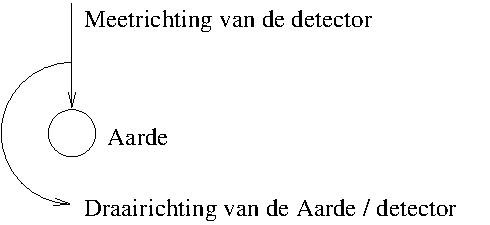
\includegraphics[scale=0.75]{opstelling}
\par\end{centering}

\caption{De Aarde in het heelal}
\end{figure}


We kunnen op de volgende manier berekenen waar de meeste kosmische
straling vandaan komt.
\begin{itemize}
\item We verdelen de hemel in vier kwadranten.
\item We berekenen hoeveel straling uit een kwadrant komt. Dit kan door
het ontbinden van een vector.
\item Tegenoverliggende kwadranten worden nu positief en negatief.
\end{itemize}
De hoek van de Aarde in radialen is te berekenen met:

\begin{equation}
\alpha=2\pi\frac{t}{T}
\end{equation}


We kunnen de omlooptijd van de Aarde nu ook de tijd ten opzichte van
de sterren nemen. Ten opzichte van de hemel draait de Aarde in 1 jaar
1 extra rondje.


\paragraph*{Opdracht 5:}

\emph{Bereken de duur van een siderische dag in zonne-uren.}

\begin{figure}[h]
\noindent \begin{centering}
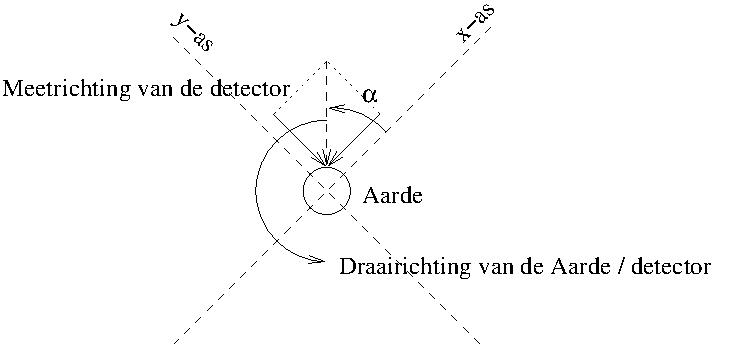
\includegraphics[scale=0.75]{opstelling1}
\par\end{centering}

\caption{Het ontbinden van de meetgegevens}
\end{figure}


We kunnen nu de meetgegevens voor ieder interval ontbinden met de
formules:

\begin{equation}
\begin{array}{c}
Data_{x}=Data*sin(\alpha)\\
Data_{y}=Data*cos(\alpha)
\end{array}
\end{equation}


of:

\begin{equation}
\begin{array}{c}
Data_{x}=Data*sin(2\pi\frac{t}{T})\\
Data_{y}=Data*cos(2\pi\frac{t}{T})
\end{array}
\end{equation}


Als de gemeten kosmische straling op ieder moment hetzelfde is, zal
de som van $Data_{x}$ en $Data_{y}$ over 1 periode $T$ altijd 0
zijn. Is er echter op een bepaald tijdstip meer kosmische straling,
dan wordt minstens ��n van beide sommen positief of negatief. Als
$Data_{x}$ positief is, dan zal er meer kosmische straling langs
de posieve x-as komen, als $Data_{y}$ positief is, dan zal er meer
kosmische straling langs de posieve y-as komen. Als de som negatief
is, komt er meer kosmische straling langs de negatieve as.

Al deze bewerkingen zijn in een spreadsheet programma te doen. Het
is echter van belang om altijd een geheel aantal periodes te gebruiken,
doe je dit niet dan krijg je een fout door het afbreken van de tijd.
Verder moet je goed controleren of de gemeten waarden juist zijn.
Is de detector bijvoorbeeld altijd aan geweest? 


\paragraph*{Opdracht 6:}

\emph{Bereken hoeveel zonne-uren je minimaal nodig hebt om een geheel
aantal siderische dagen te meten.}

We kunnen het afbreken minder zwaar mee laten wegen, door het begin
en het eind minder zwaar te laten wegen. Officieel moet dit met een
Gauss-kromme. Helaas is deze functie oneindig lang en hebben we niet
zoveel gegevens. Een Gauss-kromme is bij benadering goed te benaderen
met een ``raised cosine'': $gewicht=\frac{1}{2}(1-cos(2\pi\frac{t}{T_{m}}))$.

\begin{figure}[h]
\noindent \begin{centering}
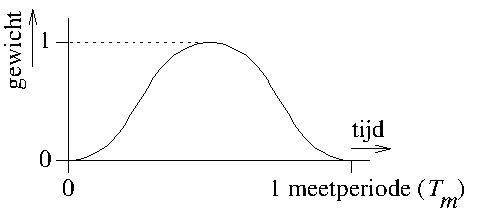
\includegraphics[scale=0.75]{raisedCosine}
\par\end{centering}

\caption{Een ``raised cosine''}
\end{figure}


De procedure wordt nu dus:
\begin{itemize}
\item Haal de gegevens van een station op.
\item Controleer of de gegevens over de periode kloppen. Is er ergens een
dip in de gegevens dan is er iets vreemds aan de hand. Bekijk de dippen
dus goed, misschien stond de detector uit.
\item Bereken de duur van een siderische dag.
\item Laat het begin en het eind van je metingen minder zwaar wegen door
de metingen met een ``raised cosine'' te vermenigvuldigen.
\item Bepaal de $Data_{x}$ en $Data_{y}$ component.
\item Tel alle $Data_{x}$ gegevens bij elkaar op. Doe dit ook voor $Data_{y}$.
\item Is de som van beide gegevens 0 dan is er geen richting waar te nemen
waarin er meer kosmische straling is.
\end{itemize}
Wat te doen als de som niet 0 is? Ik meet bijvoorbeeld voor $\sum Data_{x}=-525$
en $\sum Data_{y}=260$. Dit is natuurlijk in een assenstelsel weer
te geven:

\begin{figure}[h]
\noindent \begin{centering}
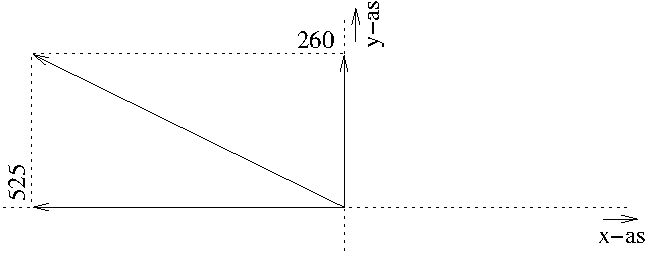
\includegraphics[scale=0.75]{resultaat}
\par\end{centering}

\caption{Het resultaat}


\end{figure}


In figuur 4.4 is de richting waaruit de kosmische straling komt te
zien. De intensiteit van de extra kosmische straling moeten we nog
vergelijken met de totale kosmische straling. Als we weten hoeveel
co�ncidenties er in het totaal in deze periode zijn geweest, is dit
vrij eenvoudig te bepalen:

\begin{equation}
afwijking=\frac{\sqrt{\sum Data_{x}^{2}+\sum Data_{y}^{2}}}{\sum Data}\%
\end{equation}

\end{document}
